\section{Entwicklung des Gesamtkonzepts} \label{sec:Meth gesamtkonzept}
Um ein Gesamtkonzept für das \gls{Modul} zur automatischen Verhaltensklassifikation zu entwerfen, sind einige grundlegende Aspekte zu betrachten. Das beinhaltet die Definition der Aufgabe, die es zu lösen gilt. Die Anforderungen die das \gls{Modul} erfüllen soll, sind zu formulieren. Ebenfalls ist zu analysieren, welche Informationen und Anwendungen für den Aufbau zur Verfügung stehen. Bezogen auf den \gls{Machine Learning Workflow} (\autoref{sec:MLWF}) handelt es sich hierbei, um die \textit{Problemdefinition} und die Vorbereitung für das \textit{Sammeln von Daten}. \par

\subsection{Anforderungen an das Modul} \label{sec:Meth Anforderungen}

Die Anforderungen an das \gls{Modul} lassen sich unter anderem aus der Zielsetzung (\autoref{sec:Zielsetzung}) ableiten. 

\begin{itemize}
    \item \textit{Modularität}: Aus der Forderung nach \glsdisp{Modul}{Modularität} entsteht die Anforderung einer einfachen Integrierbarkeit in eine Datenverarbeitungskette von übergeordneten Systemen.
    \item \textit{Echtzeitfähigkeit}: Das \gls{Modul} muss in der Lage sein, einen Datenstrom in Echtzeit zu verarbeiten. Das Klassifikationsergebnis muss vorliegen, bevor das Ereignis vorbei ist. Daraus ist die Anforderung einer möglichst kurzen Laufzeit abzuleiten.
    \item \textit{Verhaltenserkennung}: Das Verhalten der Puten soll erkannt und klassifiziert werden. Daraus ist abzuleiten, dass das \gls{Modul} ein \gls{Klassifikation}[sproblem] lösen muss.
    \item \textit{Automation}: Eine automatische Verarbeitung der Daten ist als Ziel definiert. Die Konzepterstellung muss auf eine automatische Verarbeitung ausgelegt werden. 
    \item \textit{Zeitrahmen}: Die Entwicklungsdauer des \gls{Modul}[s] darf den Zeitrahmen der Arbeit nicht überschreiten. Daraus ist abzuleiten, dass die Komplexität des Konzepts begrenzt seien sollte, um die Einhaltung des Zeitplans zu gewährleisten.
\end{itemize}


\subsection{Rohdatengrundlage und Voraussetzungen} \label{sec:Meth RohDat}
Die Rohdaten sind fundamental für den Aufbau von Anwendungen des \glsdisp{ML}{maschinellen} Lernens. Im \gls{Machine Learning Workflow} wird sich ab dem zweiten Prozessschritt mit ihnen auseinander gesetzt (\autoref{sec:Worflow DatSam}). Die frühe Position im Ablauf zeigt, dass sämtliche folgenden Prozesse auf den Rohdaten fußen. Eine frühzeitige Bestandsaufnahme der zur Verfügung stehenden Rohdaten kann einen erfolgreichen Verlauf des Workflows gewährleisten. \par

Im \acrshort{OptiLiMa} Projekt wurden Rohdaten aus einem Mastputenstall gesammelt. Dieser wurde mit 12 Kameras ausgestattet, die jeweils einen anderen Stallbereich abdeckten. Positioniert wurden die Kameras so, dass sie das Stallgeschehen in Vogelperspektive aufzeichneten. Die Abbildung \ref{fig:KamerasImStall} stellt die Einteilung des Mastputenstalls, in die mit Kameras abgedeckten Bereiche dar. Mit eingezeichnet ist der Ungefähre verlauf der Futterbahnen.

\begin{figure}[htb]
    \centering
    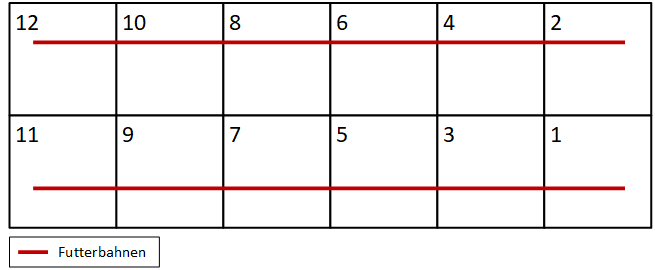
\includegraphics[width=0.9\textwidth]{img/Grafiken/Stallbereiche mit Futterbahn.png}
    \caption[Abteile des Mastputenstalls mit Verlauf der Futterbahnen.]{Abteile des Mastputenstalls mit Verlauf der Futterbahnen. Die Nummer in den oberen linken Ecken stehen für die IDs der Kameras.}
    \label{fig:KamerasImStall}
\end{figure}

Die Kameras zeichneten einen Videostream auf. Die Bildinformationen wurden verwendet, um ein \gls{Detektion}[s]\glsdisp{Modul}{modul} anzuwenden. Dieses \glsdisp{Detektion}{detektierte} und \glsdisp{Lokalisation}{lokalisierte} die Puten im \gls{Frame}. Die \gls{Detektion} verlief in Echtzeit. Die \gls{Detektion}[en] wurde in einer Datenbank gespeichert, welche sich auf einem Server befindet. Jeder Eintrag beinhaltet einen eindeutigen Zeitstempel und ein dazugehöriges \gls{Frame} in einem Videostream. Die Videostreams wurden auf Festplatten gespeichert. Insgesamt wurden  drei Mastdurchläufe aufgezeichnet. Ein Lebenszyklus der Puten umfasst ca. 4 Monate. Nach einer Aufzuchtphase von einem Monat komme die Tiere in den Mastputenstall. Ab diesem Punkt begann die Datenerfassung. \par

Die Datensammlung im Mastputenstall war bereits vor Beginn dieser Arbeit abgeschlossen. Somit ließ sich kein Einfluss auf die zur Verfügung stehende Rohdatennmenge nehmen und auch nicht auf die Art der Rohdaten. Die Videostreams liegen als im mp4-Dateiformat vor. Das direkte Arbeiten auf der Datenbank mit den \gls{Detektion}[en] ist aufgrund des Datenvolumens und der Rechenleistung der Server nicht praktikabel. Aus diesem Grund wurde ein Tool entwickelt, welches auf die Datenbank zugreift und Daten eines angegebenen Zeitintervalls herunterlädt. Die heruntergeladenen \gls{Detektion}[en] speichert das Tool in einer csv-Datei. In einer vorausgegangenen Arbeit im Rahmen des \acrshort{OptiLiMa} Projekts, ist ein \gls{Assoziation}[s]\glsdisp{Modul}{modul} aufgebaut worden. Mittels der \gls{Detektion}[en] ist so ein \gls{MOT} System aufgebaut worden. \par

Die \gls{Detektion} und die \gls{Assoziation} bauen auf dem Videostream auf. Jedes \gls{Frame} im Videostream hat einen eindeutigen Zeitstempel zugeordnet. Dadurch wird sichtlich, dass die vorhandenen Rohdaten in Form von Zeitreihen vorliegen.

\subsection{Definition der Aufgabe} \label{sec:Meth DefAufgabe}
Ziel ist es Verhaltensweisen der Mastputen zu Klassifizieren (\autoref{sec:Zielsetzung}). Um eine Aufgabe zu formulieren muss zunächst geklärt werden, was eine Verhaltensweise ist und wie sie sich erkennen lässt. In \cite{Levitis.2009} wird Tierverhalten definiert als Reaktionen von Individuen oder Gruppen, auf Reize aus ihrer Umgebung. Der Suffix \textit{-weise} oder \textit{-art} bezeichnet eine Gewohnheit \cite{duden.art}. Eine Verhaltensweise ist somit ein Muster im Verhalten. Im Vorfeld zu dieser Arbeit wurden zwei Verhaltensweisen identifiziert, welche besonders herausstechen. Diese werden hier als Kontrollgänge und Kämpfe bezeichnet. Im folgenden werden diese beiden Verhaltensweisen erläutert. \dubpar

\begin{quote}

\textbf{Kontrollgänge}\par
Der Tierhalter unternimmt täglich Kontrollgänge im Maststall. Die Tiere reagieren auf den Tierhalter, wenn dieser den Stall betritt und während seiner Bewegung durch den Stall. Dabei finden Massenbewegungen statt. Die Tiere werden aufgeschreckt und fangen an sich in Richtung des Tierhalters zu drängen. Oftmals berühigen sich die Tiere während sich der Tierhalter noch im Stall befindet. Nähert sich der Tierhalter ihrem Stallbereich werden sie jedoch oftmals wieder Aufgeschreckt und drängen sich erneut in Richtung des Tierhalters. In unmittelbarer nähe zum Tierhalter weichen die Tiere aus. Dadurch entsteht eine \gfuss{Traube} um den Tierhalter. Regelmäßig muss im Stall neues Stroh gestreut werden. Dafür muss der Tierhalter mit einem Traktor in den Stall. Das Verhalten der Tiere ist in diesem Fall jedoch sehr Ähnlich zum täglichen Kontrollgang. Die Tiere schrecken auf und drängen zum Traktor. Um den Traktor bildet sich ein \gfuss{Traube}. Eine Verhaltensweise, welche sich nur beim Streuen zeigt entsteht dadurch, dass der Traktor eine deutlich größere Fläche einnimmt und eine deutlich größere  \gfuss{Traube} einnimmt als der Tierhalter. Fährt der Traktor durch den Stall, bleibt hinter ihm eine große freie Fläche zurück. Die Tiere drängen nicht alle auf einmal auf diese freie Fläche. Einige Tiere nutzen die Fläche um dem Traktor zu folgen, anderen Tiere stürmen mit sehr dynamischen Bewegungen auf die freie Fläche und wieder andere Tiere bewegen sich gemächlich. Somit schließt sich die Fläche nach und nach wieder. Die Abbildung \ref{fig:bspKontrollg} zeigt einige Ausschnitte aus Kontrollgängen. 
\end{quote}


\begin{figure}[htb]
     \centering
     \begin{subfigure}[b]{0.4\textwidth}
         \centering
         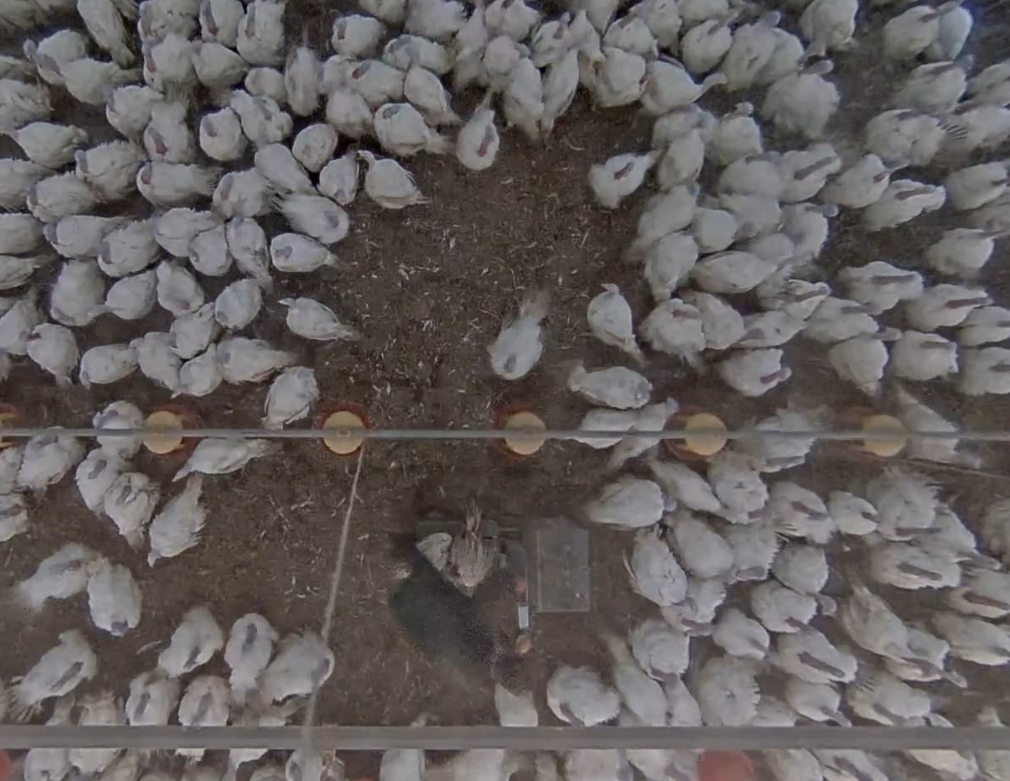
\includegraphics[width=\textwidth, height=5cm]{img/Verhaltensweisen/Kontrollgang Tierhalter Traube 2.png}
         \caption{Kontrollgang des Tierhalters.}
     \end{subfigure}
     \hfill
     \begin{subfigure}[b]{0.59\textwidth}
         \centering
         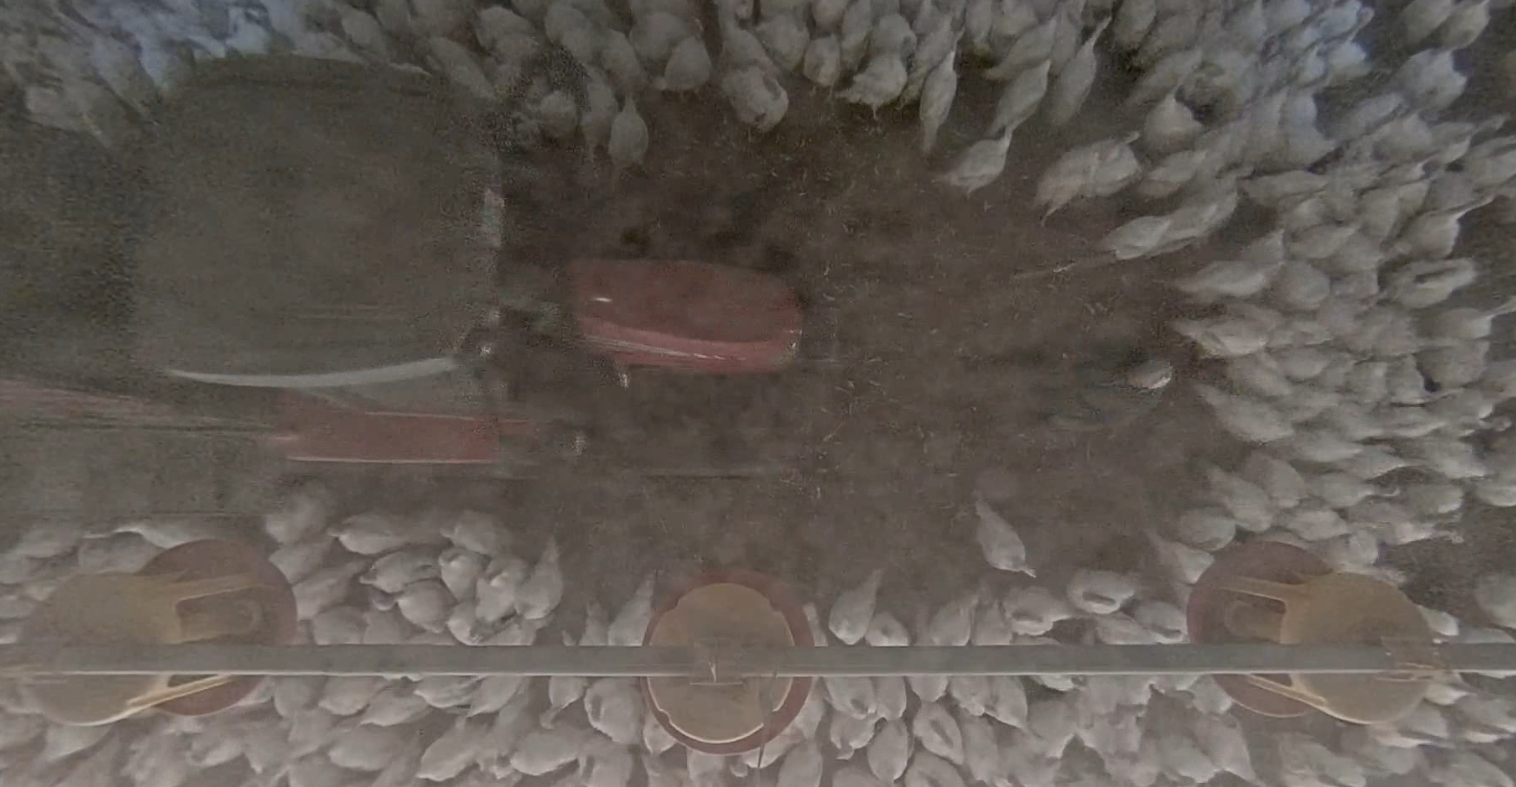
\includegraphics[width=\textwidth, height=5cm]{img/Verhaltensweisen/Kontrollgang Tracktor Traube.png}
         \caption{Einstreuung von Stroh mit Traktor.}
     \end{subfigure}
     \caption[Ausschnitte aus Kontrollgangereignissen.]{Ausschnitte aus Kontrollgangereignissen.}
     \label{fig:bspKontrollg}
\end{figure}


\par

\begin{quote}
\textbf{Kämpfe}\par
Ein Kampf entsteht ohne direkt ersichtlichen Auslöser. Anders als beim Kontrollgang, wo der Tierhalter der Auslöser ist. Ein Kampf beginnt meistens in dem sich zwei Tiere gegenüberstehen. Prüfend schauen sie ihren gegenüber an und gelegentlich versuchen sie ihn zu picken. Dies steigert sich meistens zu gegenseitigen stärkeren Pickattacken. Dabei entwickeln die Tiere eine hohe Dynamik und bewegen sich umeinander. Die umliegenden Tiere weichen den kämpfenden Tieren aus. Wodurch eine \gfuss{Traube} um die Tiere entsteht. Oft passiert es, dass eine Pute die andere packt und um sich schleudert. Dadurch entstehen zirkulierende Bewegungsmuster. Auch Verfolgungen entstehen in Kämpfen. Möchte eins der Tiere entkommen, jagd das Andere diesem oft hinterher und versucht das flüchtende Tier zu packen. Schafft es das, wird der Kampf fortgesetzt. Die Verfolgungen finden mit hoher Dynamik statt. Tiere die sich im Umfeld aufhalten weichen aus, oder werden zur Seite gedrängt. Dadurch entstehen frei Flächen im Kanal der Fluchtbewegung. Ein Kampf muss nicht nur zwischen zwei Tieren stattfinden. Auch mehrerer Tiere können an einem Kampf beteiligt sein. Ebenfalls können die kämpfenden Tiere wechseln. Z.B. schafft es ein Tier zu flüchten und der Verfolger findet dieses nicht mehr, kann es sein, dass der Verfolger auf das nächst beste Tier losgeht. Auch kann es passieren, dass ein bisher unbeteiligtes Tier dazu entscheidet mit in den Kampf einzusteigen. Enden tut der Kampf plötzlich und so wie er begonnen hat, ohne ersichtlichen Auslöser. Die Abbildung \ref{fig:bspKämpf} zeigt einige Ausschnitte aus Kämpfen.
\end{quote}

\begin{figure}[htb]
     \centering
     \begin{subfigure}[b]{0.55\textwidth}
         \centering
         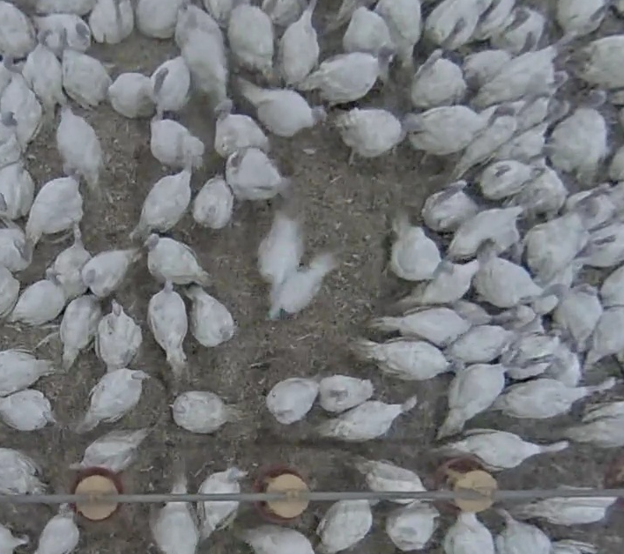
\includegraphics[width=\textwidth, height=6cm]{img/Verhaltensweisen/Kampf Traube.png}
         \caption{Kampf zwischen zwei Puten.}
     \end{subfigure}
     \hfill
     \begin{subfigure}[b]{0.44\textwidth}
         \centering
         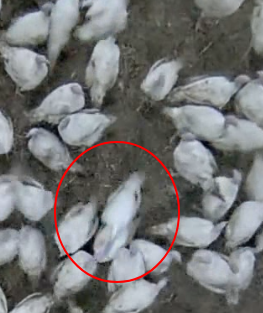
\includegraphics[width=\textwidth, height=6cm]{img/Verhaltensweisen/Kampf Verfolgung.png}
         \caption{Verfolgung eines flüchtenden Tieres.}
     \end{subfigure}
     \caption[Ausschnitte aus Kampfereignissen.]{Ausschnitte aus Kontrollgangereignissen.}
     \label{fig:bspKämpf}
\end{figure}

\par

Bei einem Kontrollgang treten dynamische Gruppenbewegungen auf, während Kämpfe durch dynmaische Bewegungen vereinzelter Tiere geprägt sind. Bezogen auf den Kameraauschnitt ist bei einem Kontrollgang Dynamik in den meisten Bildbereichen zu beobachten. Kämpfe fallen durch lokale Dynamik in vereinzelten Bildbereichen auf. \par

Für diese Arbeit wurden jegliches Verhalten was nicht in die Verhaltensweisen \textit{Kontrollgang} oder \textit{Kampf} passt, als \textit{Normalverhalten} deklariert. Der Begriff ist etwas irreführend gewählt, da \gfuss{Normalität} nicht näher definiert wurde. Jedoch sind Kämpfe und Kontrollgänge die mit Abstand auffälligsten Verhaltensweisen, deshalb wird der Fokus darauf gelegt diese Verhaltensweisen vom restlichen Verhalten im Stall abzugrenzen. Aus diesem Grund wird das restliche Verhalten als \gfuss{Normal} bezeichnet. Die Definition der Merkmale von \textit{Normalverhalten} lassen sich aus diesem Grund als Abgrenzung von den anderen beiden Verhaltensweisen Formulieren.\dubpar

\begin{quote}
\textbf{Normalverhalten}\par
Während sich ein Kontrollgang durch eine globale hohe Dynamik auszeichnet und ein Kampf durch eine lokale hohe Dynamik, sind die Tiere die meiste Zeit deutlich weniger aktiv. Bezogen auf die Bildbereiche der Kameras ist in den meisten Fällen ein Großteil der Tiere dabei sich auszuruhen. Die Tiere sitzen stationär auf einer Position. Vermehrt tritt Aktivität rund um die Futterbahnen auf. Diese ist jedoch meistens nicht so Dynamisch wie in den anderen beiden Verhaltensweisen.
\end{quote}
\par

Das Auftreten einer Verhaltensweise stellt für das geplante \gls{Modul} ein \gls{Ereignis} dar. Wie die Beschreibungen der Verhaltensweisen zeigen, basieren die charakterisierenden Merkmale vor allem auf der Bewegung der Tiere. Bewegung ist zeitabhängig. Die Merkmale der Verhaltensweise sind somit in einem Zeitraum zu beobachten und nicht zu einem Zeitpunkt. Ein \gls{Ereignis} wird also definiert durch einen Startzeitpunkt und einen Endzeitpunkt. Innerhalb dieser zeitlichen Grenzen sind die Merkmale der jeweiligen Verhaltensweise zu beobachten. \par

Aus den Anforderungen (\autoref{sec:Meth Anforderungen}) ist bekannt, dass ein \gls{Klassifikation}[sproblem] zu lösen ist. Durch die Erkenntnis, dass sich die \gls{Ereignis}[se] innerhalb eines Zeitraums abspielen und dem Fakt, dass auch die Rohdaten in Zeitreihen strukturiert sind (\autoref{sec:Meth RohDat}) wird deutlich, dass es sich bei der Aufgabe um eine \gls{Klassifikation} von Zeitreihen handelt.\par

\subsection{Aufbau des Gesamtkonzepts}
Es ist bekannt, welche Aufgabe zu lösen ist, es ist bekannt, wie die zu erkennende \gls{Ereignis}[se] aussehen, die erkannt werden sollen und es ist bekannt, welche Rohdaten zur Verfügung stehen. Mit diesem Wissen und über die Anforderungen ist ein Gesamtkonzept für das \gls{Modul} entwickelbar. Die Abbildung \ref{fig:GesKonzpt} zeigt dieses Konzept.

\begin{figure}[htb]
    \centering
    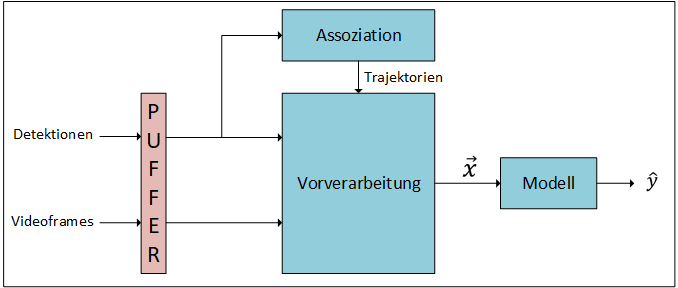
\includegraphics[width=0.9\textwidth]{img/Grafiken/Gesamtkonzept start.png}
    \caption{Gesamtkonzept des \gls{Modul}[s].}
    \label{fig:GesKonzpt}
\end{figure}


Ein Strom von Rohdaten fließt in das \gls{Modul}. Die \gls{Detektion}[sdaten] fließen in das \gls{Assoziation}\glsdisp{Modul}{smodul}. Dieses erstellt Trajektorien und gibt diese Aus. Die Rohdaten und die Trajektorien fließen in einer Vorverarbeitung zusammen. Hier werden die \gls{Feature}[s] aus den Rohdaten extrahiert und konstruiert (\autoref{sec:ML FeatExtr}), welche in der \gls{Feature}[selektion] (\autoref{sec:ML FeatSelect}) ausgewählt wurden. Nach der Vorverarbeitung wird der \gls{Featurevektor} dem ausgewählten (\autoref{sec:ML ModellSelect}), konfigurierten (\autoref{sec:ML HyperPara}) und trainierten (\autoref{sec:ML Metriken, Valid}) Modell übergeben. Dieses Schätzt, welche Verhaltensweise in der Probe zu beobachten ist und gibt ein \gls{Label} aus, welches die Klassenzugehörigkeit eindeutig bestimmt. Dieses \gls{Label} ist auch die Ausgabe des \gls{Modul}[s]. \par

Da Zeitreihen \glsdisp{Klassifikation}{klassifiziert} werden müssen und es sich dabei um sequenzielle Daten handelt, ist die Vorgehensweise für die Vorverarbeitung der Rohdaten modellabhängig (\autoref{sec:sequenzen ML}). Wie \autoref{sec:Meth Nutzwert} zeigt, besitzen die vielversprechendsten Modelle kein Sequenzverständnis. Das Modell muss als \gls{Feature}[s] erhalten, welche die Information der Zeitreihe komprimieren. Der Pufferspeicher ist dazu da die einzelnen Zeitschritte der sequentillen Rohdaten zu speichern. Sobald genügend Zeitschritte vorhanden sind, werden die Rohdaten an die Vorverarbeitung weitergegeben. Dort wird die gepufferte Sequenz zu einem einzelnen Datenpunkt komprimiert. 